\section{Results}\label{results}

Submissions to the ArgMining~2021 shared task on Quantitative Summarization and Key Point Analysis are evaluated with respect to mean average precision~(mAP)~\todocite~\todo{Cite shared task overview paper}.
The organizers calculate the score by pairing each argument with the best matching key point according to the predicted matching probabilities.
Within each topic-stance combination, only the 50\,\% of arguments with the highest predicted matching score are then considered for evaluation.
The task organizers claim that this removal of 50\,\% of the pairs is sensible because some arguments do not match any of the key points, thus would influence mean average precision negatively~\todocite.
For the remaining argument key point pairs in each topic-stance combination, average precision is calculated and the final score is computed as the mean of all average precision scores.

The task organizers now consider two variants of ground-truth labels: strict labels and relaxed labels.
Both variants are based on the ground-truth labels from the ArgKP dataset~\cite{Bar-HaimEFKLS2020}. But as the ArgKP dataset contains argument key point pairs with undecided labels~(i.e. not enough agreement between annotators), the shared task organizers derive strict labels by considering those pairs as no match, and relaxed labels by considering them as match~\todocite.
To compute each evaluation score, the strict score is calculated based on strict ground-truth labels and the relaxed score based on relaxed ground-truth labels~\todocite.

We stress that in the complex evaluation setup of the mean average precision score, the relaxed mAP score would favor assuming matches in case of model uncertainty while the strict mAP on the opposite would favor assuming no match.
Though, as only the most-probable matching key point is being considered for evaluation, this effect is minor.
The evaluation score in general favors matchers that can match a single key point for each argument with high precision.
It is however not important if a matcher does predict non-matches with high certainty.

\subsection{Automatic Evaluation}
\begin{table*}
  \centering
  \caption{Performance of the random and token overlap baseline, \BertBase, and \RobertaBase models with respect to mean average precision~(mAP), precision, and recall of the match label. We report scores for the training, validation, and test set in the strict~(S) and relaxed~(R) label settings, as well as the averages of the two settings~(\(\varnothing\)). The best result per set is highlighted \textbf{bold}.}
  \label{table-results}
  \smaller
  \setlength{\tabcolsep}{2.5mm}
  \begin{tabularx}{\linewidth}{X>{\hspace{1.0em}}ccc<{\hspace{1.0em}}>{\hspace{1.0em}}ccc<{\hspace{1.0em}}>{\hspace{1.0em}}ccc}
    \toprule
    \textbf{Approach} & 
    \multicolumn{3}{c}{\textbf{mAP}} & 
    \multicolumn{3}{c}{\textbf{Precision}} & 
    \multicolumn{3}{c}{\textbf{Recall}} \\
    \cmidrule(l{1em}r{1em}){2-4} \cmidrule(l{1em}r{1em}){5-7} \cmidrule(l{1em}){8-10}
    & S & R & \(\varnothing\) & 
    S & R & \(\varnothing\) & 
    S & R & \(\varnothing\) \\
    \midrule
    \multicolumn{10}{X}{\textit{Training set}} \\
    \midrule
    Random & 
    0.260 & 0.409 & 0.335 & 
    0.173 & 0.330 & 0.252 & 
    0.500 & 0.501 & 0.501 \\
    Token Overlap & 
    0.541 & 0.653 & 0.597 & 
    0.269 & 0.435 & 0.352 & 
    0.323 & 0.275 & 0.299 \\
    \BertBase & 
    0.889 & \textbf{0.981} & 0.935 & 
    \textbf{0.703} & \textbf{0.936} & \textbf{0.819} & 
    \textbf{0.864} & \textbf{0.607} & \textbf{0.736} \\
    \RobertaBase & 
    \textbf{0.915} & 0.979 & \textbf{0.947} & 
    0.702 & 0.927 & 0.814 & 
    0.820 & 0.572 & 0.696 \\
    \midrule
    \multicolumn{10}{X}{\textit{Validation set}} \\
    \midrule
    Random & 
    0.232 & 0.430 & 0.331 & 
    0.180 & 0.364 & 0.272 & 
    0.523 & 0.524 & 0.524 \\
    Token Overlap & 
    0.643 & 0.802 & 0.722 & 
    0.219 & 0.416 & 0.317 & 
    0.390 & 0.366 & 0.378 \\
    \BertBase & 
    0.717 & 0.928 & 0.822 & 
    0.397 & 0.648 & 0.522 & 
    \textbf{0.802} & \textbf{0.649} & \textbf{0.725} \\
    \RobertaBase & 
    \textbf{0.879} & \textbf{0.984} & \textbf{0.932} & 
    \textbf{0.567} & \textbf{0.816} & \textbf{0.692} & 
    0.799 & 0.569 & 0.684 \\
    \midrule
    \multicolumn{10}{X}{\textit{Test set}} \\
    \midrule
    Random & 
    0.237 & 0.355 & 0.296 & 
    0.150 & 0.286 & 0.218 & 
    0.545 & 0.549 & 0.547 \\
    Token Overlap & 
    0.483 & 0.575 & 0.529 & 
    0.232 & 0.350 & 0.291 & 
    0.225 & 0.178 & 0.201 \\
    \BertBase & 
    0.827 & 0.940 & 0.883 & 
    0.326 & 0.526 & 0.426 & 
    \textbf{0.848} & \textbf{0.721} & \textbf{0.784} \\
    \RobertaBase & 
    \textbf{0.913} & \textbf{0.967} & \textbf{0.940} & 
    \textbf{0.490} & \textbf{0.716} & \textbf{0.603} & 
    0.741 & 0.569 & 0.655 \\
    \bottomrule
  \end{tabularx}
\end{table*}

In Table~\ref{table-results}, we report mean average precision for strict and relaxed labels of the training, validation, and test set in the ArgKP dataset.
We complement the mAP scores by adding precision, recall, and F1 scores of the match label, both in the strict and relaxed label setting.
To aggregate results with strict and relaxed ground-truth labels we also report the average score of the two variants.
The reported scores should allow for automated and unbiased evaluation of our models and easier comparison with competitive approaches.
We report all 36~scores for the term-overlap baseline model as well as for the fine-tuned \BertBase and \RobertaBase models.
To make our results more comparable, we add a second baseline, where matches between arguments and key points of same topic and stance are predicted with uniform random probability.
That random baseline represents a worst-case matcher and any weak matcher should exceed it's evaluation scores.

\todo{Discuss results for \Roberta model and baseline.}

\subsection{Manual Error Analysis}

\begin{figure*}[t]
    \caption{ Plotted density of \Roberta and \Bert based approaches on training and development set predicted scores.}
    \label{fig:density}
    \centering
    \begin{subfigure}[b]{0.475\textwidth}
        \centering
        \subcaption{\Bert on training set}
        \label{subfig:bert_train}
        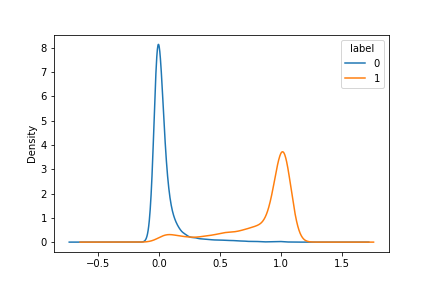
\includegraphics[width=\textwidth]{bert_train_df.png}
    \end{subfigure}
    \hfill
    \begin{subfigure}[b]{0.475\textwidth}
        \centering
        \subcaption{\Bert on development set}
        \label{subfig:bert_dev}
        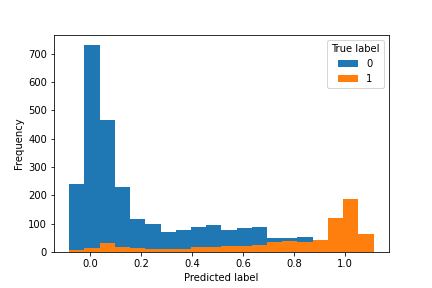
\includegraphics[width=\textwidth]{bert_dev_df.png}
    \end{subfigure}
    \vskip\baselineskip
    \begin{subfigure}[b]{0.475\textwidth}
        \centering
        \subcaption{\Roberta on training set}
        \label{subfig:roberta_train}
        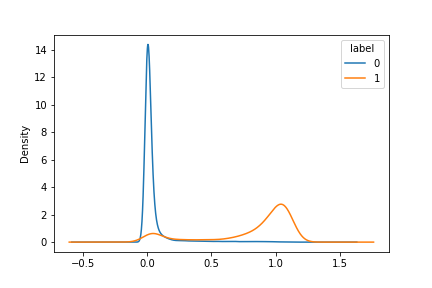
\includegraphics[width=\textwidth]{roberta_train_df.png}
    \end{subfigure}
    \hfill
    \begin{subfigure}[b]{0.475\textwidth}
        \centering
        \subcaption{\Roberta on development set}
        \label{subfig:roberta_dev}
        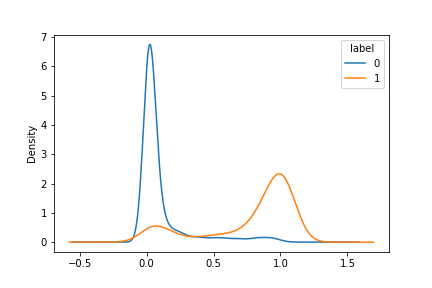
\includegraphics[width=\textwidth]{roberta_dev_df.png}
    \end{subfigure}
\end{figure*}

Plotting the density curves, shown in Figure \ref{fig:density}, of the given distributions of scores, predicted by our proposed approaches, provides 
insight about possible errors and therefore possible improvements.\\
As can be seen, the majority of predictions prove to be correctly, hence seeing obvious spikes in all four density
curves around $0$ and $1$.\\
It can also be seen that, predictions on the training set performe better than on the development set for both 
\Roberta and \Bert, concluding that better generalization is needed.\\
In Figures \ref{subfig:bert_train} and \ref{subfig:roberta_train} it's noticeable that
both approaches tend to predict better for non-matching arguments and key points on the training set. A possible explanation 
could be the higher amount of non-matching pairs provided. Most arguments match with only a few, if 
not only a single key point, but they get compared to all other key points, hence creating an imbalance in the distribution 
of data to learn from. It's possible to think of a more balanced approach, where providing the same amount of matching and 
non-matching key points for a given argument could resolve this problem.\\
Keeping an eye on the performance at the training set, we can further identify, that for matching arguments and key points, 
scores from \Bert tend to be spread more than scores from \Roberta.

Investigating Figures \ref{subfig:bert_dev} and \ref{subfig:roberta_dev} reveals that \Bert seems to have a problem with 
predicting certain non-matching and matching pairs. For example: \\

\begin{figure}[H]
    \begin{tabularx}{\linewidth}{lp{0.7\linewidth}}
            ARG: & \texttt{School uniforms can be less comfortable than students' regular clothes.}\\
            KP: & \texttt{School uniforms are expensive.}\\
            Score:& $0.479004$\\
    \end{tabularx}
\end{figure}

poses a problem for it. Possibly because this argument has no matching key point given. Hence it's imaginable that 
\Bert doesn't know how to handle it and therefore gives it a score arround $0.5$.

It's also striking, that \Bert predictes a bunch of matching argument and key point pairs as non-matching. For example, 
it seems to be very difficult to predict for the key point: \texttt{Affirmative action reduces quality.} A lot of 
arguments are quite long:\\

\begin{figure}[H]
    \begin{tabularx}{\linewidth}{lp{0.7\linewidth}}
            ARG: & \texttt{affirmative action can lead to people who are less qualified getting positions they would otherwise not be able to achieve}\\
            ARG: & \texttt{affirmative action discriminates the majority, preventing skilled workers from gaining employment over someone less qualified but considered to be a member of a protected minority group.}
    \end{tabularx}
\end{figure}

,thus beeing in total contrast to the length of the key point. Therefore it seems to be quite challenging to reduce 
such long arguments, filled with a lot of information, to very compact key points. And indeed, 
calculating the Arithmetic Mean of the difference of matching key point and argument lengths reveals, that 
for all wrongly predicted labels (Score $< 0.5$) the mean difference is $75.55$ characters while 
correctly predicted labels (Score $> 0.5$) have a mean difference of $66.59$ characters.

\Roberta reports a similar indication for matching pairs (wrong predictions: $70.09$, correct predictions: $67.93$ ), 
it could thus be assumed that character difference is a general problem for both approaches. 

In contrast to \Bert, \Roberta performes way better when it comes to predicting non-matching pairs
almost reproducing a similar performance as on the training set.

% \todo{Find example errors from our classifier. How can we improve?}
